% Schematic redraw of the printed regular triangular prism and marked points.
% E and F are placed at the stated edge ratios; projected edge lengths are not data.
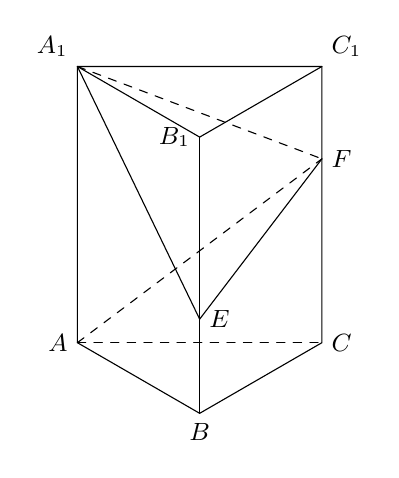
\begin{tikzpicture}[scale=1.15,line join=round,line cap=round,
  every node/.style={font=\small}]
\coordinate (A) at (0,0);
\coordinate (B) at (1.35,-.78);
\coordinate (C) at (2.7,0);
\coordinate (Aone) at (0,3.05);
\coordinate (Bone) at (1.35,2.27);
\coordinate (Cone) at (2.7,3.05);
\coordinate (E) at (1.35,.26);
\coordinate (F) at (2.7,2.03);
% Prism edges; AC is hidden in the source projection.
\draw (A)--(Aone)--(Cone)--(C)--(B)--(A);
\draw (Aone)--(Bone)--(Cone);
\draw (B)--(Bone);
\draw[dashed] (A)--(C);
% Question construction lines and hidden diagonals as printed.
\draw (Aone)--(E)--(F);
\draw[dashed] (A)--(F) (Aone)--(F);
\node[left] at (A) {$A$};
\node[below] at (B) {$B$};
\node[right] at (C) {$C$};
\node[above left] at (Aone) {$A_1$};
\node[left] at (Bone) {$B_1$};
\node[above right] at (Cone) {$C_1$};
\node[right] at (E) {$E$};
\node[right] at (F) {$F$};
\end{tikzpicture}
